\documentclass[a4paper]{report}
\usepackage[T1]{fontenc}
\usepackage[utf8]{inputenc}
\usepackage[english]{babel}
\usepackage{titlesec}
\usepackage{lipsum}
\usepackage{booktabs}
\usepackage{hyperref}
\usepackage{graphicx}
\usepackage{float}
\graphicspath{ {./img/} }

\begin{document}

%%The two following lines remove the line "Chapter n" at the beginning of each chapter, before the title
%\titleformat{\chapter}[display]
%  {\normalfont\bfseries}{}{0pt}{\Large}
\titleformat{\chapter}[hang] 
{\normalfont\huge\bfseries}{\thechapter}{1em}{} 

\author{Nicola Rosetti \and Simone Sartoni \and Vittorio Torri}
\title{Safe Streets}
\date{}
\maketitle

\tableofcontents

\chapter{Introduction}
\section{Scope}
SafeStreet is an application meant to provide a mechanism to more efficiently detect parking violations and to try to make streets safer. This is meant both for normal people and for municipality agents. 
The application domain concerns different types of world phenomena, shared phenomena and machine phenomena. \\
We can identify the following world phenomena:
\begin{itemize}
\item {[W1]} A car is illegally parked 
\item {[W2]} An accident occurs
\item {[W3]} An intervention is performed to make the roads safer
\end{itemize} 
the following shared phenomena controlled by the world and observed by the machine:
\begin{itemize}
\item {[S1]} A violation report is sent by a user
\item {[S2]} An accident report is provided by the municipality system
\end{itemize}
and the following shared phenomena controlled by the machine and observed by the world:
\begin{itemize}
\item {[S3]} A traffic ticket is emitted by an agent, exploiting the municipality system, after a report analysis
\item {[S4]} An agent is sent to verify the correctness of a violation report
\item {[S5]} A suggestion for a safety improvement on streets is made available
\end{itemize}

\section{Purpose}
The following are the goals of the system:

\section{Definitions, acronyms and abbreviations}
\begin{itemize}
\item \textit{GPS}: Global Positioning System
\end{itemize}
\section{Revision history}
\lipsum[1]
\section{Reference documents}
\lipsum[1]
\section{Document structure}
\lipsum[1]

\chapter{Overall Description}
\section{Product perspective}
In figure \ref{fig:class-diagram} is reported an \textit{UML Class Diagram} which represents the domain of the application with main concepts and data involved, including their relationships.\\
Not all classes will necessary become effective classes in the implementation (e.g. the \textit{Visitor} class).\\
Some data appear to be duplicated in the \textit{TrafficTicket} class but it needs to be considered the fact that the application will receive also data about traffic tickets which have not been issued as a consequence of a SafeStreet report, but instead have been independently issued by the local police in their traditional control activities. They are necessary to correctly build statistics and they need to include data which are already present in the corresponding report, when it exists.\\
For what concerns the \textit{Accidents} here it has been supposed a representation for all types of accidents, coming from the municipality data, then the system will be able to discriminate the ones related to parking violations.\\
In figure [...] is reported an \textit{UML State Diagram} to clearly represent the state evolution of a \textit{ViolationReport}, which is the main object which change its state during time, while the other ones do not present significant evolutions from this point of view.
\begin{figure}[hp]
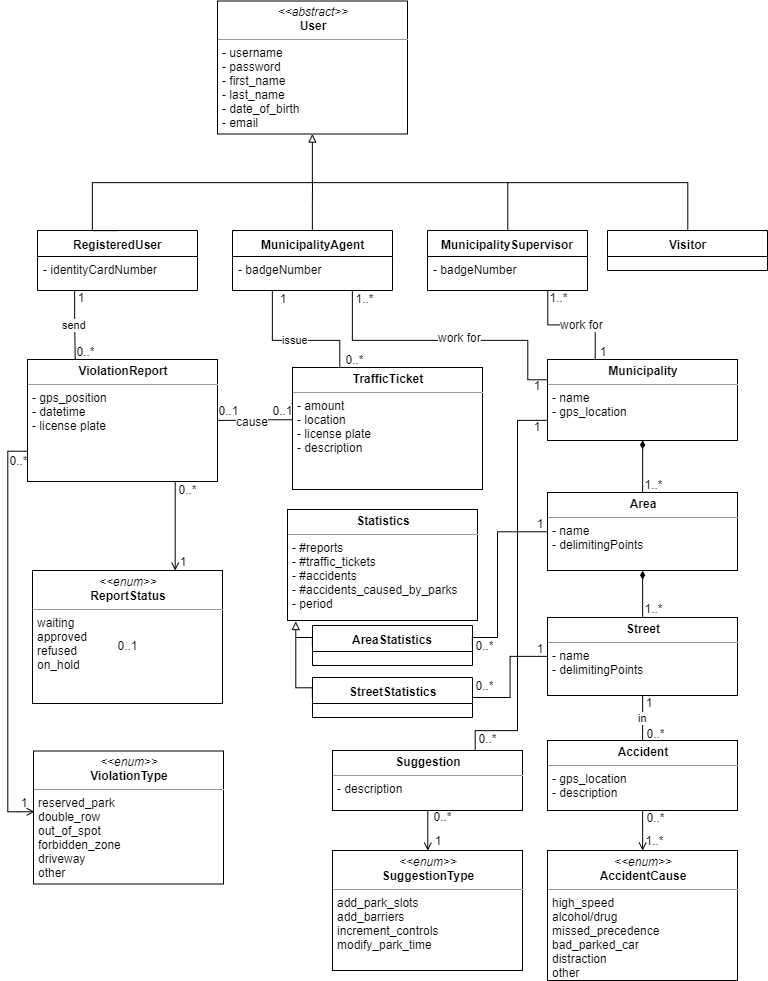
\includegraphics[width=\textwidth]{ClassDiagram}
\caption{UML Class Diagram}
\label{fig:class-diagram}
\end{figure}

\section{Product functions}
In this part are underlined the main functions offered by SafeStreet, divided by the users that can actually have access to them.

\subsection{Visitor}

\subsubsection{Registering to the application}

The system offers the possibility to Visitors to register and actually become users of the application. When registering the visitor needs to provide his name, surname, birthdate, fiscal code and identity card number. They are mandatory so if some of them is not provided then the registration process fails.
 
\subsection{User}

\subsubsection{Reporting a violation}
This is the most important function offered by SafeStreets. This function allows Users, when logged in, to report a potential violation that has occured in the streets. 
They can achieve that by inserting some mandatory data. When reporting a violation, a user must insert the type of violation that has been detected ( missing park disk, car illegally parked in the bike lane, car illegally parked in some reserved parking spot, not paid parking disk).
Subsequently, the user must provide at least one picture of the violation. Through the pictures, the user should provide clear evidence of the violation and the vehicle involved (in particular the license plate) before sending the report for a verification to the server. Optionally, the user can help recognition providing the license plate of the vehicle as plain text. Before sending the report, the application attaches to it the current position of the User (using GPS position), date and time of the report (taken through the network).

\subsection{Municipality agent}
\subsubsection{Authority agent registering}
Differently from the function previously explained and meant for normal Users, this function is only meant for Municipality agents. Each agent (tipically a maximum of 3 per municipality) can register to SafeStreet to exploit his services as agent. He needs to provide his name, surname, birthdate and rank. After providing a password, the registration is sent for a verification to the municipality service and completed if the data inserted is correct. An ID code is then given to the agent to be uniquely identified.

\subsubsection{Violation checking}

This function is provided if and only if the municipality involved has installed the service needed to exploit SafeStreet data. After logging in as a municipality agent, the system notifies the agent about all the current not resolved reported violations. The agent can visualize individually each report, checking if the report corresponds to an actual violation. He can  either directly emit a traffic ticket or send an agent directly on the street to check and eventually emit the ticket.
Additionally, when logged in, the agent is notified of new incoming reports.

//TODO nico 


\subsection{Municipality supervisor}

\subsubsection{Suggesting possible solutions} 
This function consists of a task periodically executed by the system (e.g. once a month) which tries to analyze reported violations, issued tickets, accidents information and data about the streets network coming from the municipality to suggest possible interventions to increase the safety (e.g. add barriers, create new park spots, increase the allowed parking time, send more agents in a certain area in certain hours...). When the system finds new suggestions it sends them to the municipality supervisors.

\subsubsection{Getting sensible information}
This function allows logged in municipality supervisors to retrieve information about the vehicles with the highest number of violations in a selected area. The system must return information belonging to the supervisor's area of competence, communicated during the registration process.

\subsection{Everyone} 

\subsubsection{Consulting statistics}
This function allows visitors, users, municipality agents or supervisors to retrieve information about the streets and areas with the highest frequency of violations; it is possible to retrieve statistics and trends about the accidents correlated to the parking violations, the effectiveness of SafeStreet initiatives and the issuing of traffic tickets. The information provided must be mined by the system from the reported violations, crossed with information from municipality. The system must not allow user to see confidential data about other people; it must allow the user to choose a topic: areas with most accidents, areas with the highest number of traffic tickets issued or areas where there have been the best improvements and in the end the system must show to the user the information about the topic selected.



\section{User characteristics}
The users of the service are the following:
\begin{itemize}
\item \textit{Visitor}: a non-logged user which can only consult statistics about areas with the highest frequency of violations, highest rate of accidents related to the violations, traffic tickets issued and safety improvements. 
\item \textit{User}: an identified user which, in addition to the \textit{visitor}, can report a parking violation, sending the details to the municipality authorities.
\item \textit{Municipality agent}: an agent of the local police which is notified about the violation reports for his municipality and can decide whether to immediately send a traffic ticket to the person responsible for a certain violation or to send an agent on the place to verify it and possibly discard it.
\item \textit{Municipality supervisor}: he has a full access to the application data, including all statistics and the suggestions to improve safety in the most dangerous areas.
\end{itemize}
\section{Assumptions, dependencies and constraints}
\subsection{Dependencies and constraints}
\label{SS-Dep&Const} 
The presence of some services provided by the municipalities is necessary to make all SafeStreet functions operative. In particular the following services are requested:
\begin{itemize}
\item \textit{Identity Card Check}: allows to retrieve data of a person given its identity card number.  It's request for a strong user authentication.
\item \textit{Accidents Information}: return information about the accidents occurred in the municipality streets, with position and causes.
\item \textit{Traffic Ticket Issue}: allows to send traffic tickets to a certain person by a certain agent
\item \textit{Agents Identity Check}: allows to check the identity of a registering agents given his personal data, including his badge number. 
\end{itemize}
\subsection{Domain Assumptions}
\lipsum[1]

\chapter{Specific Requirements}
\lipsum[1]
\section{External interface requirements}
\subsection{User Interfaces}
\lipsum[1]
\subsection{Hardware Interfaces}
No hardware interfaces are provided, being SafeStreet just a software system.
\subsection{Software Interfaces}
The system does not provide any software interface, because there are no other application which actually need to retrieve data from it. \\
The system has to call the municipalities services to retrieve some information (see \ref{SS-Dep&Const} ).
\subsection{Communication Interfaces}
The communication between users and SafeStreet servers exploit internal APIs through the \textit{HTTPS} protocol. The same is assumed for the communication with the municipalities systems. \\
For the \textit{users} the communication is unidirectional, in the sense that they cannot receive requests/notification by the server, all communications start from them. \\
The \textit{municipality agents} can be notified from the server when there are new report to be analyzed. \\
The \textit{municipality supervisors} can be notified about suggestions for interventions on the most unsafe areas.
\section{Functional requirements}
\lipsum[1]
\section{Performance requirements}
Performance requirements are not particularly critical for the system, but it is anyway desirable that all requests sent to the server are answered within 1 second, to assure a good user experience. \\
The server infrastructure will be designed to be scalable so that it will be possible to adapt it to the increment of users when the app diffusion will increase.
\section{Design constraints}
%\subsection{Standards compliance}
\subsection{Regulatory policies}
The application will only record the data strictly correlated to the reported violations and the data provided by the users during the registration. This data will be used only for the purposes of the system and will be treated confidentially, according to the \textit{GPDR} rules.\\
In particular the statistical analyses performed will never show publicly any information which can be related to a specific person.
\subsection{Hardware and software limitations}
The following requirements are necessary to install the mobile application:
\begin{itemize}
\item \textit{Operating system}: Android 5+ or iOS 9+
\item \textit{Hardware}: to allow the access as logged user the smartphone needs to have a camera and a GPS sensor
\end{itemize}
The camera is needed to take photos of the violations and the GPS is necessary to automatically record the position. The users have to give the relative permissions to the application. A base necessary requirement to use any functionality is the presence of an internet connection.\\
This requirements allow the majority of people to use the application \mbox{(see \hyperref[ref:os-stats]{\textit{[OS-STAT]}}).}\\
The authorities have the possibility to use a web interface, accessible through every modern browser.\\
Everyone can consult the publicly available statistics also through the \textit{SafeStreet website}, with any modern browser.
\subsection{Any other constraints}
//PROBABLY NOTHING
\section{Software system attributes}
\subsection{Reliability-Availability}
The availability is not a critical requirement, but the system has to guarantee a 99\% of uptime (max 3.65 days/year of downtime) to ensure that the users can normally use it.
\subsection{Security}
Security is a critical requirement for this system, considering the confidential information that are transmitted through it. It is assured by the use of the \textit{HTTPS} protocol for all communications and by the follow of the best security practices for the servers management, protecting them with IDS, maintaining the data ciphered and assuring the access only to the authorized users. \\
Every activity performed by municipality agents and supervisors will be logged to ensure its traceability.
\subsection{Maintainability}
The system will be realized following the best software engineering practices to ensure its maintainability and expandability in the future.
\subsection{Portability}
The system is actually designed to be compatible with most of Android and iOS devices (smartphones and tablets) and from the authorities side it can be accessed from any web browser, so it is very portable.
It will be important to maintain it compatible with the future releases of this two operating systems and with any other new operating system or device that will acquire an important market share.
\chapter{Formal Analysis using Alloy}
\lipsum[3]

\chapter{Effort spent}

\begin{center}
Nicola Rosetti \\
%\begin{tabular}{lll}
\begin{tabular}{p{2cm}p{1.5cm}p{7cm}}
\toprule
\textit{Date} & \textit{Hour} & \textit{Section} \\ \midrule
17-10-2019 & 1.5 h* & Goals \\
\bottomrule
\end{tabular}
\end{center}
\vspace*{1 cm}
\begin{center}
Simone Sartoni \\
\begin{tabular}{p{2cm}p{1.5cm}p{7cm}}
\toprule
\textit{Date} & \textit{Hour} & \textit{Section} \\ \midrule
17-10-2019 & 1.5 h* & Goals \\
\bottomrule
\end{tabular}
\end{center}
\vspace*{1 cm}
\begin{center}
Vittorio Torri \\
\begin{tabular}{p{2cm}p{1.5cm}p{7cm}}
\toprule
\textit{Date} & \textit{Hour} & \textit{Section} \\ \midrule
17-10-2019 & 1.5 h* & Goals \\ \midrule
20-10-2019 & 1 h & Users, Hardware and software limitations, goal refinement \\ \midrule
21-10-2019 & 1 h & Software, Hardware and Communication Interfaces, Performance requirements, Design constraints, Software system attributes \\ \midrule
22-10-2019 & 1 h & Goal and requirements revision \\ \midrule
23-10-2019 & 1 h & Goal and requirements revision \\ \midrule
26-10-2019 & 2 h & Scenarios, requirements, functions, scope \\ \midrule
28-10-2019 & 1.5 h & Product perspective and UML Class Diagram \\
\bottomrule
\end{tabular}
\end{center}
\textit{* Group work}

\chapter{References}
\begin{itemize}

\item \label{ref:os-stats} [OS-STAT] \href{https://gs.statcounter.com}{\textit{https://gs.statcounter.com}} - statistics on operating systems market share and versions diffusion

\item \label{ref:slander} [SLANDER] see art. 368, 370 and 69 c.p.p. (Italian law)

\end{itemize}

\end{document}
